\documentclass[11pt]{article}
\usepackage{lindrewlite}

\title{\textbf{Matching People to Jobs}\\[2pt]\large The theory, the code, and the report behind Delta Code 2026, Problem Statement 1}
\author{Notes for a curious reader (no prior graph theory needed)}
\date{October 2026}

\begin{document}
\maketitle
\tableofcontents
\bigskip

\begin{plain}
This document explains, from scratch, everything behind the project: \emph{why} a quick-and-easy way of handing out jobs leaves people unplaced, \emph{what} mathematics fixes it, \emph{how} the program \code{allocate.py} carries that mathematics out, and \emph{how to read} the three outputs (\code{assignment.csv}, \code{matching\_vis.png}, \code{report.md}). Gold boxes like this one restate the idea in everyday language.
\end{plain}

%=====================================================================
\section{The problem: who gets which job?}\label{sec:problem}

A company has \textbf{2{,}400 candidates} and \textbf{320 roles}. Each role has a limited number of seats (between 3 and 10), and each candidate is only eligible for a few roles (1 to 5). We want to place \emph{as many candidates as possible}, with nobody in a role they are not eligible for and no role over its seat limit.

This is the same puzzle as residency placements, assigning jobs to servers in a data centre, or seating guests so everyone gets a table they are happy with.

\subsection{The tempting shortcut: ``first come, first served''}

The obvious method, called \textbf{greedy}, goes through the candidates one by one and puts each into the first eligible role that still has a seat. It is fast and easy to explain. But every decision is final, and that is its weakness.

\begin{example}{The smallest trap}{trap}
Two roles, each with one seat: $X$ and $Y$. Two candidates:
\begin{itemize}[nosep]
 \item \textbf{Ann} is eligible for $X$ and $Y$ (she lists $X$ first).
 \item \textbf{Ben} is eligible for $X$ only.
\end{itemize}
Greedy handles Ann first and gives her $X$. Now Ben arrives: $X$ is full and he cannot do $Y$, so \textbf{Ben is left out}. Total placed: 1. But if Ann had taken $Y$, \emph{both} would have a job. Total possible: 2.
\end{example}

\begin{figure}[h]
\centering
\begin{tikzpicture}[every node/.style={font=\small},cand/.style={circle,draw=lin-blue,fill=lin-blue!15,minimum size=8mm},role/.style={rectangle,draw=lin-gold,fill=lin-gold!20,minimum size=8mm}]
 % greedy
 \node[cand] (a1) at (0,1) {Ann}; \node[cand] (b1) at (0,0) {Ben};
 \node[role] (x1) at (2.6,1) {X}; \node[role] (y1) at (2.6,0) {Y};
 \draw[gray] (a1)--(y1); \draw[gray] (b1)--(x1);
 \draw[very thick,lin-red] (a1)--(x1);
 \node at (1.3,-0.9) {\textbf{Greedy:} 1 placed (Ben stranded)};
 % optimal
 \node[cand] (a2) at (7,1) {Ann}; \node[cand] (b2) at (7,0) {Ben};
 \node[role] (x2) at (9.6,1) {X}; \node[role] (y2) at (9.6,0) {Y};
 \draw[gray] (a2)--(x2);
 \draw[very thick,lin-green] (a2)--(y2); \draw[very thick,lin-green] (b2)--(x2);
 \node at (8.3,-0.9) {\textbf{Optimal:} 2 placed};
\end{tikzpicture}
\caption{Thick lines are the chosen placements. Ann moving from $X$ to $Y$ ``makes room'' for Ben.}
\end{figure}

\begin{keyidea}
Greedy fails because it never \emph{reconsiders}. The cure is a systematic way of saying: ``if someone stuck needs a seat, can we shift a chain of already-placed people, each one step, so a seat opens up?'' That chain is called an \textbf{augmenting path}, and it is the star of this project.
\end{keyidea}

On the project's data, greedy places \textbf{1{,}709} candidates while the best possible is \textbf{1{,}901}. The difference, \textbf{192 people}, is the \emph{Greedy Capacity Gap} that the problem statement asks us to measure.

%=====================================================================
\section{Graphs and matchings}

\begin{definition}{Graph, bipartite graph}{graph}
A \textbf{graph} is a set of dots (\emph{vertices}) joined by lines (\emph{edges}). It is \textbf{bipartite} if the dots split into two teams so that every line joins a dot of one team to a dot of the other. Here the teams are $U$ (candidates) and $V$ (roles); a line $u$--$v$ means ``candidate $u$ is eligible for role $v$''.
\end{definition}

\begin{definition}{Matching}{matching}
A \textbf{matching} $M$ is a set of edges in which no vertex is used twice. In words: every candidate gets at most one role and (in the simplest case) every role at most one candidate. Its size $|M|$ is the number of edges. A \textbf{maximum matching} is one with the largest possible size.
\end{definition}

\subsection{Roles with several seats}

Real roles have capacity $c_v$ (the number of seats). The standard trick is to \textbf{split a role into $c_v$ identical slots}: a role with 3 seats becomes three one-seat roles, each connected to the same candidates. A capacity-respecting assignment is then just an ordinary matching in the bigger graph, so all matching theory applies unchanged. (The program does not literally make copies; it uses capacities directly, as explained in Section~\ref{sec:flow}.)

\begin{plain}
A matching is a legal set of placements. ``Maximum'' means: no legal set places more people.
\end{plain}

%=====================================================================
\section{Augmenting paths and Berge's Lemma}\label{sec:berge}

Fix a matching $M$ (say, the one greedy produced). Call a vertex \textbf{free} if $M$ does not use it (an unplaced candidate, or an empty seat).

\begin{definition}{Augmenting path}{aug}
An \textbf{$M$-augmenting path} is a path that
\begin{enumerate}[nosep]
 \item starts at a free candidate and ends at a free seat, and
 \item alternates: a line \emph{not} in $M$, then a line in $M$, then not in $M$, \dots, ending with a line not in $M$.
\end{enumerate}
\end{definition}

In the trap example the path is: \emph{Ben} $\to X$ (not in $M$) $\to$ \emph{Ann} (this is the line Ann--$X$, in $M$) $\to Y$ (not in $M$, and $Y$ is a free seat). Reading it as a story: ``Ben takes $X$, Ann leaves $X$ and takes $Y$.''

\textbf{Flipping} the path means: lines that were in $M$ go out, lines that were out come in. Every person on the path ends up placed (the two ends gain a partner, the middle people just swap), so the matching grows by exactly one:
\[
 |M_{\text{new}}| = |M| + 1 .
\]

\begin{theorem}{Berge's Lemma}{berge}
A matching $M$ is maximum \textbf{if and only if} there is no $M$-augmenting path.
\end{theorem}

\begin{plain}
If a ``shift-everyone-one-step'' fix exists, you are not done. If no such fix exists \emph{anywhere}, you have the best possible answer. So the recipe is: keep finding fixes until none are left.
\end{plain}

\begin{proof}
($\Rightarrow$) If an augmenting path exists, flipping it gives a legal matching one larger, so $M$ was not maximum.

($\Leftarrow$) Suppose $M$ is not maximum; let $M'$ be a bigger matching. Draw only the lines that are in exactly one of $M$ and $M'$; call this picture $H$. Each dot touches at most one line of $M$ and at most one of $M'$, so in $H$ every dot touches at most 2 lines. Hence $H$ falls apart into separate paths and loops, and along each, lines alternate between $M$ and $M'$. Loops and even-length paths have equally many $M$ and $M'$ lines. Since $|M'|>|M|$, some piece has \emph{more} $M'$ lines; it must be an odd-length path that begins and ends with $M'$ lines. Take an end dot $x$. Its single line in $H$ is an $M'$ line. If $M$ also touched $x$ by some line $e$, then $e\notin M'$ (as $M'$ uses only one line at $x$), so $e$ would lie in $H$ and give $x$ two lines in $H$, a contradiction. So both ends are free for $M$, and the piece is an $M$-augmenting path.
\end{proof}

%=====================================================================
\section{Flow networks: a plumbing view}\label{sec:flow}

Finding augmenting paths cleverly is easiest in the language of \emph{flows}, which you can picture as water in pipes.

\begin{definition}{The network $G'$}{net}
Add two new dots: a \textbf{source} $s$ and a \textbf{sink} $t$. Add pipes
\begin{itemize}[nosep]
 \item $s\to u$ with capacity $1$, for every candidate $u$ (each person is placed at most once);
 \item $u\to v$ with capacity $1$, for every eligible pair;
 \item $v\to t$ with capacity $c_v$, for every role $v$ (its number of seats).
\end{itemize}
\end{definition}

Pushing one unit of water from $s$ to $t$ along $s\to u\to v\to t$ means ``place candidate $u$ in role $v$''. The \textbf{maximum flow} (the most water you can push) equals the \textbf{maximum number of hires}.

\begin{figure}[h]
\centering
\begin{tikzpicture}[every node/.style={font=\small},dot/.style={circle,draw,minimum size=7mm},cand/.style={dot,draw=lin-blue,fill=lin-blue!15},role/.style={dot,draw=lin-gold,fill=lin-gold!20},>=Stealth]
 \node[dot,fill=black!8] (s) at (0,0) {$s$};
 \node[cand] (a) at (2.4,0.9) {Ann}; \node[cand] (b) at (2.4,-0.9) {Ben};
 \node[role] (x) at (5.2,0.9) {$X$}; \node[role] (y) at (5.2,-0.9) {$Y$};
 \node[dot,fill=black!8] (t) at (7.6,0) {$t$};
 \draw[->] (s)--node[above,sloped]{1}(a); \draw[->] (s)--node[below,sloped]{1}(b);
 \draw[->] (a)--node[above]{1}(x); \draw[->] (a)--node[near start,above,sloped]{1}(y); \draw[->] (b)--node[below]{1}(x);
 \draw[->] (x)--node[above,sloped]{$c_X{=}1$}(t); \draw[->] (y)--node[below,sloped]{$c_Y{=}1$}(t);
\end{tikzpicture}
\caption{The trap example as a network. The most water that can flow from $s$ to $t$ is 2.}
\end{figure}

\subsection{The residual graph: ``what can still change?''}

After some water is flowing, draw the \textbf{residual graph}: a pipe with spare room can still carry more (forward), and a pipe carrying water can have its water \emph{pushed back} (backward). A path from $s$ to $t$ in this residual picture is exactly an augmenting path. A backward step $X\to$ Ann reads ``Ann gives up $X$''.

\begin{theorem}{Max-flow = min-cut}{mfmc}
The largest possible flow equals the smallest total capacity of any set of pipes whose removal disconnects $s$ from $t$ (a \emph{cut}).
\end{theorem}

\begin{plain}
There is always a bottleneck. If the program ends with no route left from $s$ to $t$, the set of dots still reachable from $s$ marks the bottleneck, and its capacity is exactly the number of hires. That is a second, independent proof of optimality. On our data both numbers are \textbf{1{,}901}.
\end{plain}

%=====================================================================
\section{Doing it fast: Hopcroft--Karp (Dinic's idea)}\label{sec:fast}

Finding one augmenting path at a time works but can be slow. Hopcroft and Karp's improvement is to find \emph{many shortest fixes at once}. Each \textbf{phase} has two steps:

\begin{enumerate}
 \item \textbf{BFS (levels).} Starting at $s$, label every dot by how many steps away it is, using only pipes with spare room (like ripples spreading on a pond). If $t$ never gets a label, there are no fixes left: \textbf{stop, we are optimal}.
 \item \textbf{DFS (blocking flow).} Using only pipes that go from level $k$ to level $k{+}1$, repeatedly walk from $s$ towards $t$, push one unit along each path found, and update. Dead ends are remembered and never tried again in this phase. Continue until no such walk exists.
\end{enumerate}

Then repeat. After each phase, the length of the shortest remaining fix strictly grows.

\begin{plain}
First fix everyone who can be fixed with a short shuffle, then those needing longer shuffles, and so on. In our run the shuffle lengths were 5, 7, 9, 11 steps, and only \textbf{four phases} were needed.
\end{plain}

\subsection{How many steps does it take?}

Let $N$ be the number of dots in the network and $|E|$ the number of pipes.

\textbf{One phase costs about $|E|$.} The BFS touches each pipe once. In the DFS each pipe is a dead end at most once, and each pipe (except the last ones into $t$) has capacity 1, so it carries at most one path per phase.

\textbf{There are only about $\sqrt N$ phases.} After $\sqrt N$ phases every remaining fix is at least $\sqrt N$ steps long. Each person can be used by only one fix at a time (they have a single unit of throughput), so the leftover fixes are \emph{disjoint}, and each uses at least $\sqrt N/2$ people. At most $N/(\sqrt N/2)=2\sqrt N$ of them fit, and every phase handles at least one. So at most about $\sqrt N$ more phases.

\[
 \text{total time}\;\approx\; \underbrace{O(\sqrt N)}_{\text{phases}} \times \underbrace{O(|E|)}_{\text{per phase}} = O(|E|\sqrt{|V|}).
\]

\begin{remark}
The \emph{guarantee} is generous; reality is kinder. For 2{,}400 candidates $\sqrt N\approx 52$ phases would be the worst case, but only 4 were needed because the greedy start was already close to optimal.
\end{remark}

%=====================================================================
\section{The same problem as a table of equations (linear algebra view)}\label{sec:ilp}

The title of this problem says ``Linear Algebra'', so here is that view. Give every eligibility line $e=(u,v)$ a variable $x_e$ that is $1$ if we use it and $0$ otherwise. Then:
\begin{align*}
 \text{maximise}\quad & \sum_e x_e \quad(\text{total hires})\\
 \text{subject to}\quad & \sum_{e\ni u} x_e \le 1 \quad\text{for each candidate } u \quad(\text{at most one job}),\\
 & \sum_{e\ni v} x_e \le c_v \quad\text{for each role } v \quad(\text{seat limit}),\\
 & x_e\in\{0,1\}.
\end{align*}
Written as $A\mathbf x\le \mathbf b$, the matrix $A$ has one row per candidate and per role and one column per eligibility line; each column has exactly two ones (its candidate row and its role row). This is the \textbf{Integer Linear Program (ILP)}.

If we allow $0\le x_e\le 1$ to be fractions, we get the \textbf{LP relaxation}, which is much easier to solve. In general fractions can cheat, but for bipartite matching the matrix $A$ is \textbf{totally unimodular}: every square sub-table has determinant $0$, $+1$ or $-1$, which forces the best LP solution to consist of whole numbers anyway. That is why, in the benchmark, LP, ILP and our flow method all report exactly 1{,}901.

\begin{plain}
The ``spreadsheet of constraints'' version and the ``water in pipes'' version are two descriptions of the same problem. The spreadsheet solver is general-purpose; the pipes solver is specialised, so it is faster (about 3--4 times, in our tests).
\end{plain}

%=====================================================================
\section{Reading the code: \texttt{allocate.py}}

The program is one file, built from small functions. Below, each piece is shown and explained in everyday terms.

\subsection{Making the data}

\begin{lstlisting}
def generate(seed=2026, n_cand=2400, n_roles=320):
    rng = random.Random(seed)
    caps = [rng.choice([3, 4, 5, 6, 7, 8, 10]) for _ in range(n_roles)]
    w = [1.0 / (i + 1) ** 0.7 for i in range(n_roles)]   # popularity
    rng.shuffle(w)
    ...
\end{lstlisting}
No real data came with the problem, so the program invents some \emph{reproducibly}: the same ``seed'' always gives the same data. Seat counts are random; some roles are made more popular than others (that is realistic, and it is exactly what hurts greedy). Each candidate gets 1--5 eligible roles, in order of preference. The result is saved as \code{data\_edges.csv} and \code{data\_roles.csv}. To use real data, run the program with \code{--edges} and \code{--roles} instead.

\subsection{The greedy baseline}

\begin{lstlisting}
def greedy(cand_adj, caps):
    load = [0] * len(caps)
    match = [-1] * len(cand_adj)
    for u, nb in enumerate(cand_adj):
        for v in nb:
            if load[v] < caps[v]:
                match[u] = v
                load[v] += 1
                break
    return match
\end{lstlisting}
\code{load[v]} counts how many seats of role $v$ are taken. For each candidate $u$ (in order), look through their roles; take the first one with a free seat; the \code{break} means ``decision made, never revisited''. \code{-1} means ``not placed''.

\subsection{Building the pipe network}

\begin{lstlisting}
def _add(self, a, b, c):
    e = len(self.to)
    self.to += [b, a]
    self.cap += [c, 0]
    self.adj[a].append(e)
    self.adj[b].append(e + 1)
    return e
\end{lstlisting}
Every pipe is stored \emph{together with its reverse pipe}, in neighbouring slots $e$ and $e{+}1$. The forward pipe starts with capacity $c$; the reverse starts with $0$. Pushing one unit through a pipe means \emph{lowering} its capacity by 1 and \emph{raising} its partner's by 1; that is how ``pushing water back'' (undoing a placement) is allowed. The partner of pipe \code{e} is \code{e \textasciicircum{} 1} (flip the last bit of the number): a compact trick.

The network constructor then creates pipes $s\to$ candidates (capacity 1), candidate $\to$ role for each eligibility line (capacity 1), and role $\to t$ (capacity $c_v$), exactly as in Definition~\ref{def:net}.

\subsection{Starting from greedy (warm start)}

\code{push\_initial} pre-loads the greedy placements into the network, as if water were already flowing along them. This matters for the report: every fix the algorithm then finds is a genuine \emph{repair of a greedy mistake}, which is what lets us print ``how greedy misallocations were undone''.

\subsection{Step 1 of each phase: BFS levels}

\begin{lstlisting}
def bfs(self):
    level = [-1] * self.n
    level[self.s] = 0
    q = deque([self.s])
    while q:
        x = q.popleft()
        for e in self.adj[x]:
            y = self.to[e]
            if self.cap[e] > 0 and level[y] < 0:
                level[y] = level[x] + 1
                q.append(y)
    return level
\end{lstlisting}
\code{level} is the ``ripple distance'' from the source; \code{-1} means not reached yet. We only walk along pipes with room left (\code{cap[e] > 0}). If the sink ends with level \code{-1}, no fix exists.

\subsection{Step 2 of each phase: DFS blocking flow}

\begin{lstlisting}
def blocking_flow(self, level, trace):
    it = [0] * self.n
    flow = 0
    s, t = self.s, self.t
    while True:
        path, x = [], s
        while x != t:
            moved = False
            while it[x] < len(self.adj[x]):
                e = self.adj[x][it[x]]
                y = self.to[e]
                if self.cap[e] > 0 and level[y] == level[x] + 1:
                    path.append(e); x = y; moved = True
                    break
                it[x] += 1
            if not moved:
                if x == s:
                    return flow
                level[x] = -1          # dead end: prune
                e = path.pop(); x = self.to[e ^ 1]
                it[x] += 1
        for e in path:
            self.cap[e] -= 1; self.cap[e ^ 1] += 1
        flow += 1
        trace.append([self.to[e ^ 1] for e in path] + [t])
\end{lstlisting}
This is a walk from $s$ towards $t$ that only steps ``one level deeper''. \code{it[x]} remembers which pipe at dot $x$ we try next, so no pipe is tried twice. If we get stuck, we mark the dot as a dead end and step back. When we reach $t$, we flip the pipes along the path (\verb|cap[e] -= 1; cap[e ^ 1] += 1|), count one more hire, and save the path in \code{trace}; these saved paths become the ``chains'' in the report. When even $s$ is stuck, the phase is over.

\subsection{The main loop and reading the answer}

\code{run()} alternates BFS and blocking flow until BFS cannot reach $t$; that moment is the proof of optimality (Berge). \code{extract()} then reads off who ended up where: a candidate-to-role pipe that is full (capacity 0) means ``this candidate is placed in this role''.

\subsection{Checks and benchmarks}

\begin{itemize}
 \item \code{verify\_feasible}: confirms every placement is eligible and no role exceeds its seats.
 \item \textbf{Min-cut check}: finds everything still reachable from $s$ and adds up the capacity of pipes leaving that set; the program asserts it equals the number of hires.
 \item \textbf{networkx}: only to compute the max-flow value independently, and to draw the picture. The matching itself uses none of it.
 \item \textbf{scipy}: \code{milp} solves the ILP of Section~\ref{sec:ilp} and \code{linprog} the LP; both are timed against our method on four growing data sizes.
\end{itemize}

\subsection{The tests}

\code{test\_allocate.py} builds 300 small random puzzles, solves each by our method (with and without the greedy warm start), and demands that the result is legal, equals networkx's answer, and leaves no augmenting path. It also re-checks the main data set (1{,}901 hires).

\subsection{How to run}

\begin{lstlisting}[language=bash]
pip install -r requirements.txt
python test_allocate.py        # prints: all tests passed
python allocate.py             # writes all outputs
\end{lstlisting}

%=====================================================================
\section{Reading the outputs}

\subsection{\texttt{assignment.csv}}

One row per candidate (2{,}400 rows). Columns: \code{candidate\_id}; \code{role\_id} (empty if unplaced); \code{status} (\code{ASSIGNED} or \code{UNASSIGNED}); \code{greedy\_role\_id} (what greedy had given them); \code{changed\_vs\_greedy} ($1$ if the optimal plan moved them, which happened to 251 people who switched roles plus the 192 newly placed people that greedy had left out, 443 rows in all). Of the 2{,}400 candidates, 1{,}901 are placed and 499 are not: at that point no further reshuffling can help, because every route from them to a free seat is blocked (this is exactly the bottleneck found by the min-cut).

\subsection{\texttt{matching\_vis.png}}

\begin{figure}[h]
\centering
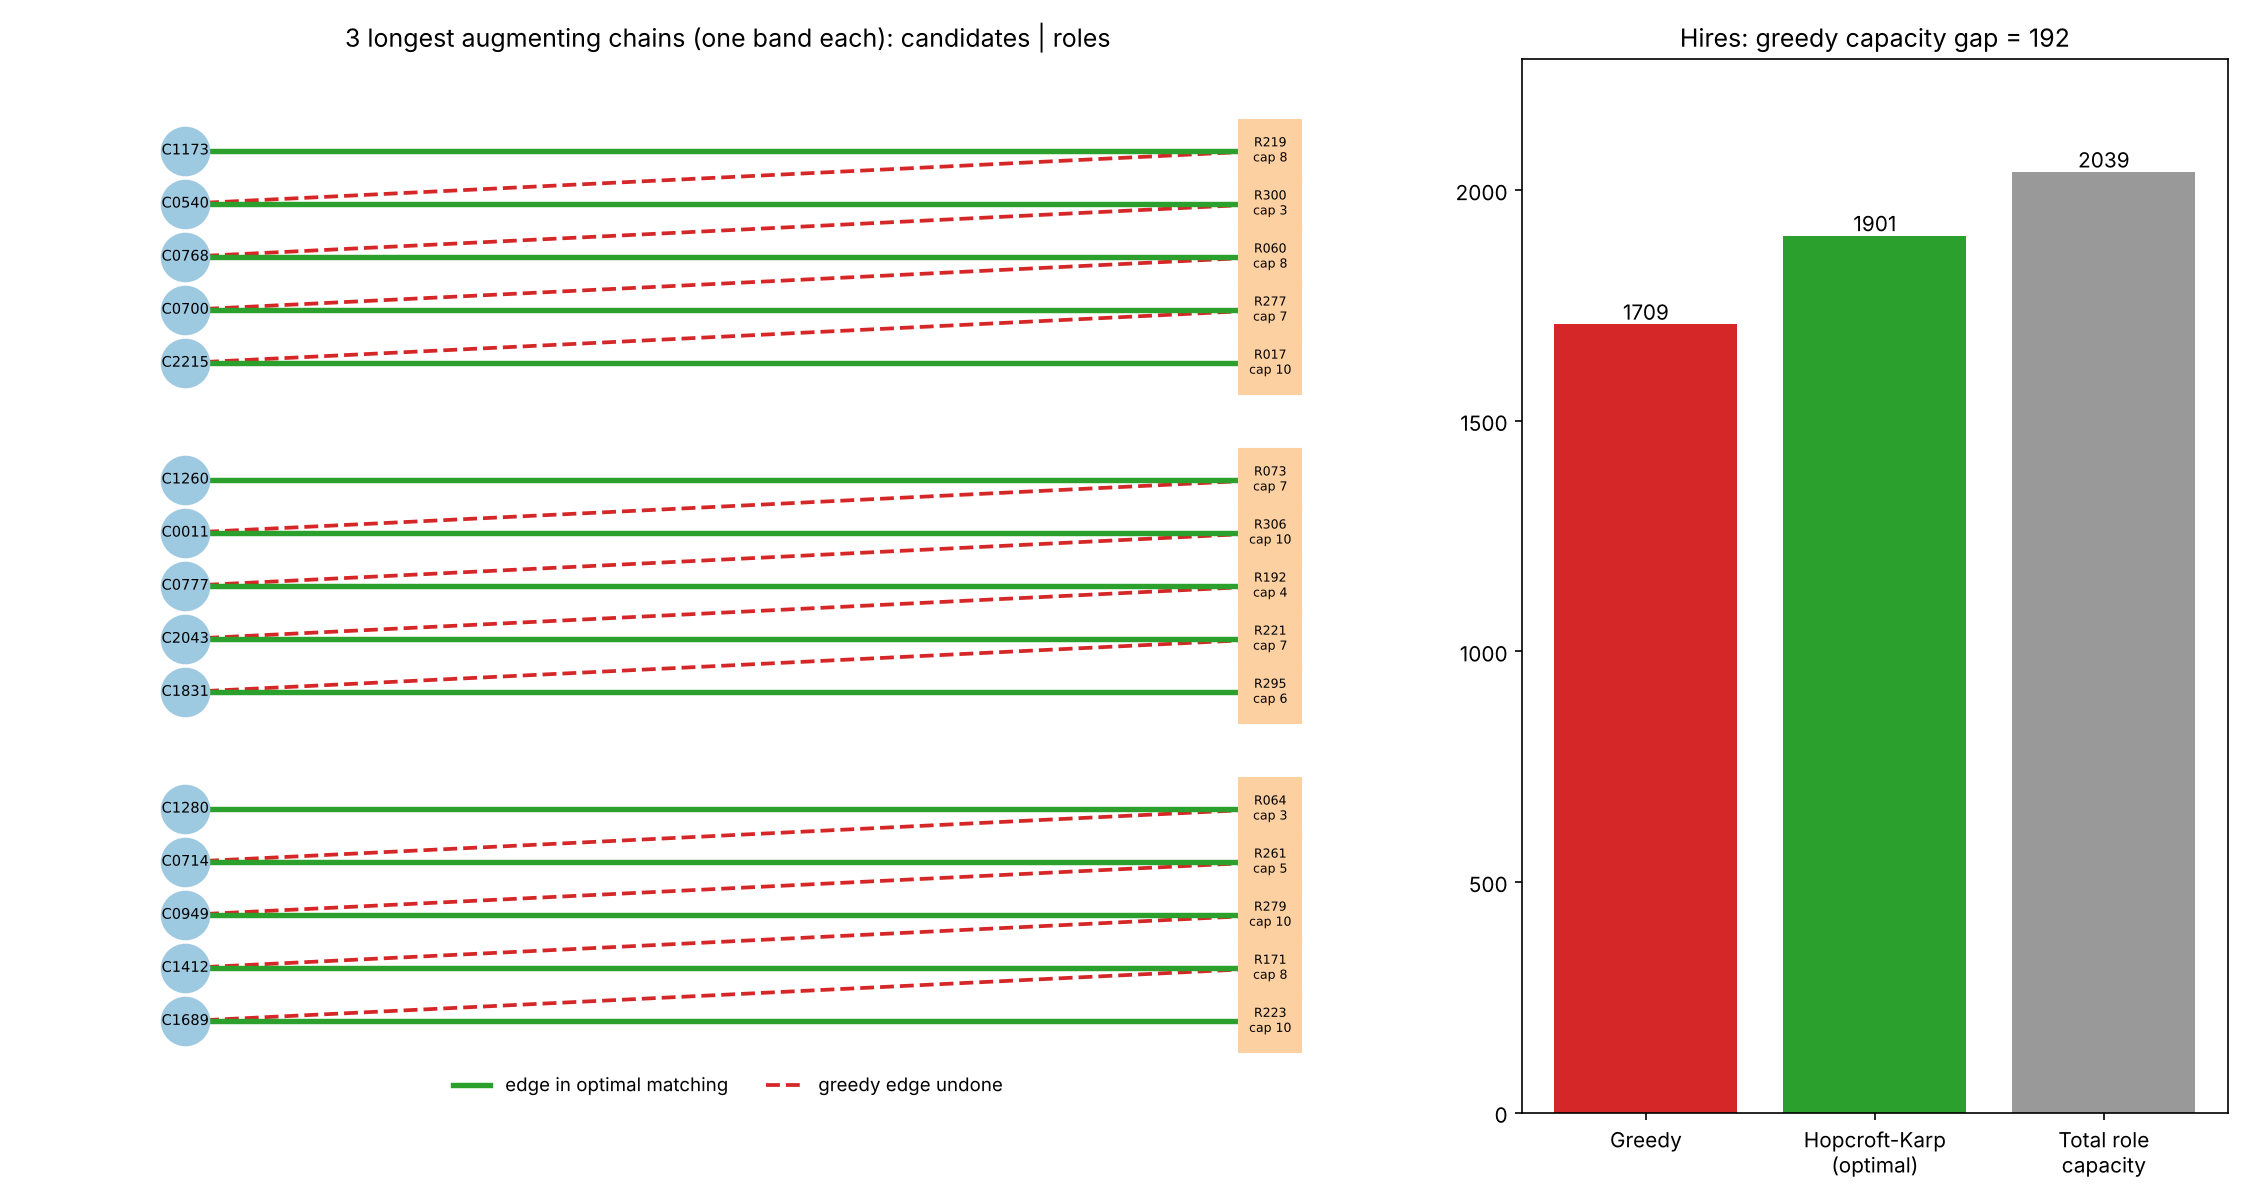
\includegraphics[width=\linewidth]{matching_vis.png}
\caption{The project's figure. \textbf{Left:} three of the longest repair chains, one per horizontal band. Candidates on the left, roles on the right. A red dashed line is a placement greedy made that the algorithm \emph{undid}; a green line is a placement in the final optimal plan. Each candidate's red line ends at the role that the next candidate down the chain takes: this staircase is the ``everybody shifts one seat'' story. \textbf{Right:} hires achieved by greedy (1{,}709), by the optimal method (1{,}901), and the total seats on offer (2{,}039).}
\end{figure}

Why not draw everything? With 2{,}400 candidates a full picture is an unreadable hairball, so the figure shows representative chains instead.

\subsection{\texttt{report.md}}

The report is the written argument. Its sections:
\begin{enumerate}[nosep]
 \item \textbf{Setup}: data sizes and the pipe-network model (Sections~\ref{sec:problem}--\ref{sec:fast} here).
 \item \textbf{Results}: greedy 1{,}709 versus optimal 1{,}901, so the gap is \textbf{192} (11.2\% more than greedy). networkx, ILP and LP all agree.
 \item \textbf{Berge's Lemma and optimality proof}: the proof from Section~\ref{sec:berge}, plus the certificate that no fix remains and the cut equals 1{,}901.
 \item \textbf{Complexity} $O(|E|\sqrt{|V|})$: the argument of Section~\ref{sec:fast}.
 \item \textbf{Path traces}: step-by-step stories of repair chains, e.g.\ ``C1173 takes R219, C0540 vacates R219 and takes R300, \dots, C2215 takes R017 (a free seat)''. Five placements and four removals give a net of \emph{one extra person hired}, with nobody losing their job.
 \item \textbf{Benchmark}: our method took about 25\,ms; the ILP took about 123\,ms. As the data doubles three times (to 9{,}600 candidates), our time grows roughly like $|E|^{1.27}$, well within the theory.
 \item \textbf{Takeaways and caveats}: especially that the data is synthetic.
 \item \textbf{Reproduce}: the commands.
\end{enumerate}

\begin{example}{Reading one repair chain}{chain}
``C1173 takes R219 $\to$ (C0540 vacates R219) $\to$ C0540 takes R300 $\to$ (C0768 vacates R300) $\to$ \dots''. Phrases without parentheses are \emph{new} placements; phrases in parentheses are people \emph{leaving} a seat greedy gave them (backward pipes). Count the ``takes'': five placements; count the ``vacates'': four removals; net $+1$ hire.
\end{example}

%=====================================================================
\section{Glossary and a quick self-check}

\begin{center}\small
\begin{tabular}{@{}p{3.1cm}p{10.4cm}@{}}
\toprule
\textbf{Term} & \textbf{Meaning in this project}\\\midrule
Greedy & Place each candidate in the first open eligible role; never reconsider.\\
Matching & A legal set of placements.\\
Free vertex & An unplaced candidate or an unfilled seat.\\
Augmenting path & A chain of shifts that places one more person.\\
Berge's Lemma & No augmenting path $\Leftrightarrow$ the matching is the largest possible.\\
Flow / network & Water-in-pipes model; max flow = max hires.\\
Residual graph & Pipes showing what can still be added or undone.\\
BFS / DFS & Level labelling / walking one level deeper at a time.\\
Phase & One BFS plus one blocking-flow round.\\
Min-cut & The bottleneck; its capacity equals the maximum flow.\\
ILP / LP & Spreadsheet-style formulation (whole numbers / fractions allowed).\\
Greedy Capacity Gap & Optimal hires minus greedy hires (here 192).\\
\bottomrule
\end{tabular}
\end{center}

\subsection*{Self-check questions}
\begin{enumerate}
 \item In the Ann--Ben example, write the augmenting path and say what flipping it does.
 \item Why does greedy get stuck but the augmenting-path method does not?
 \item What single fact tells the program it can stop?
 \item Why is the LP answer a whole number here?
 \item Why was the \emph{warm start} from greedy useful for the report?
\end{enumerate}
\textit{Answers.} (1)~Ben$\to X\to$Ann$\to Y$: Ben takes $X$, Ann moves to $Y$; one more person placed. (2)~Greedy never undoes a choice; the method can reverse placements along a chain. (3)~The BFS cannot reach the sink: no augmenting path remains (Berge). (4)~The constraint table is totally unimodular. (5)~Every fix found is then a repair of a specific greedy decision, which can be narrated.

\end{document}
